\documentclass[a4paper, oneside, 11pt]{report}
\usepackage[a4paper, vmargin=1.0cm, top=0.5cm, bottom=2.0cm, headsep=1.0cm, nofoot ]{geometry}
\usepackage[utf8]{inputenc}      			% kodowanie literek
\usepackage[polish]{babel}				% reguły dla języka polskiego
\usepackage[OT4]{fontenc}				% ładne czcionki w PDFie
\usepackage{polski}					% polski
\usepackage{indentfirst} 				% wcięcia pierwszego akapitu
\usepackage{anysize}
% \usepackage{wrapfig} 					% oblewanie rysunków tekstem
\usepackage[pdftex]{graphicx} 				% dołączanie obrazków - tryb pdftex

\makeindex
\date{}
%\date{06.12.2007 r.} %wyłšczenie drukowania daty
%----------------------------------------------------------------------------
\begin{document}
\begin{titlepage}
\begin{center} 
\textsf{} \\[2cm]
\rule{14cm}{1mm} \\
\textsf{\huge Rozproszona baza danych\\ \large Dokumentacja projektu} \\
\rule{14cm}{1mm} \\
\textsf{Piotr Kalański, Marcin Kubacki, Marek Kurdej, Adrian Wiśniewski} \\
\vspace{3cm}
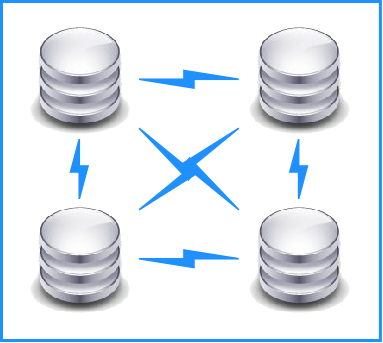
\includegraphics[width=10cm]{under_title.png}
\end{center}
\end{titlepage}

\selectlanguage{polish} 		% wybierz polski
\pagestyle{headings}
\tableofcontents
\chapter{Wprowadzenie}
Obecnie redundancja w systemach bazodanowych jest koniecznością. Zabezpiecza ona przed utratą danych, gdyby z pewnych powodów pojedynczy węzeł odmówił posłuszeństwa. Rozwiązaniem typowym w środowiskach produkcyjnych jest klaster wysokiej dostępności (ang. emph{High Availability Cluster}), który powiela transakcje na poszczególnych węzłach. 

Tematem projektu było stworzenie rozproszonej bazy danych, a właściwie klastra wysokiej dostępności, która umożliwiałaby wykonywanie zapytań na dowolnym węźle, a następnie automatyczną synchronizację takiej operacji na pozostałe węzły bazy. Dodatkowo w przypadku uruchomienia nowego węzła, węzeł ten powinien móc zsynchronizować się z pozostałymi węzłami. 

Ze względu na ograniczenia czasowe rozwiązanie zostanie przedstawione na 2 implementacjach zamiast 4, pierwszej napisanej w języku Java oraz drugiej w .NET. Trzecia implementacja w Qt nie funkcjonowała poprawnie, więc zostanie wykluczona z dalszych rozważań.

Kluczowymi algorytmami rozproszonymi dla tego projetu były:
\begin{itemize}
	\item trójfazowe zatwierdzanie transakcji (ang. \emph{Three Phase Commit})
	\item autorski pomysł synchronizacji dynamicznie dołączanych węzłów
\end{itemize}
Oba algorytmy zostaną szczegółowo omówione w dalszej części dokumentacji. Dodatkowo, aby łatwiej można było wgłębić się w niektóre części kodu - przedstawiono również diagramy sekwencji.
\chapter{Architektura}
Całe rozwiązanie składa się z kilku części. Ogólnie podzielić projekt można na następujące warstwy:
\begin{itemize}
	\item komunikacyjną
	\item logiki aplikacyjnej
	\item dostępu do danych
\end{itemize}
\section{Warstwa komunikacyjna}
W skład warstwy komunikacyjnej wchodzą klasy służące do nasłuchiwania na wybranym porcie TCP i UDP. Nasłuchiwanie na porcie TCP potrzebne jest do odbierania dowolnych komunikatów obsługujących transakcje, natomiast UDP używany jest w celu odbierania tzw. "heartbeats", czyli komunikatów wysyłanych w regularnych odstępach przez wszystkie węzły w celu ogłaszania wszystkim zainteresowanym, że dany węzeł jest dostępny. Po odebraniu żądania połączenia tworzona jest obiekt klasy roboczej - TCP Worker, który zajmuje się odbieraniem pakietów i składaniem wiadomości w całość. Następnie każdy z wątków zajmujący się takimi połączeniem przekazuje wiadomość do Dispatcher'a.

Ostatecznie po przetworzeniu wiadomości musi nastąpić pewna reakcja obiawiająca się wysłaniem konkretnego pakietu. I tu używane są klasy TCP i UDP sender, które wysyłają wcześniej przygotowaną wiadomość. Tu warto jeszcze wspomnieć o Hello generatorze, który okresowo wysyła heartbeats (i tylko on korzysta z protokołu UDP). Ważny jest tu TCP sender, który przechowuje pulę połączeń, ewentualnie nawiązuje nowe.

\section{Warstwa logiki aplikacyjnej}
Dispatcher odpowiada za klasyfikację wiadomości i odpowiednią reakcję. Reakcja ta obiawia się utworzeniem odpowiedniej klasy roboczej, która będzie odpowiadała za przechodzenie po grafie stanów automatu trójfazowego zatwierdzania transakcji, lub synchronizacji węzłów. W zależności od tego, czy węzeł w danym momencie koordynuje transakcję, czy realizuje polecenia z innych węzłów tworzone są instancje obiektów Cohort lub Coordinator - podobnie dla synchronizacji (przedrostek Restore). W obu przypadkach użyto wzorca projektowego ,,Stan''.

Każda z klas nadzorująca daną sesję, kontroluje czas spędzony w oczekiwaniu i ewentualnie powiadamia o upłynięciu limitu czasu na odpowiedź.

\section{Warstwa dostępu do danych}
W tej warstwie znajdują się wszelkie klasy, które mają na celu manipulować właściwymi danymi przechowywanymi w bazie. Klasą, która po części jest logiką aplikacyjną jest Database state. Ma ona na celu przechowywać aktualne blokady i stan bazy danych. Oprócz tego występują dwie inne pomocnicze klasy - Database connector i SQL parser, które mają na celu parsować i zapytania i umożliwiać dialog z właściwą bazą danych.

Każde z zapytań jest wstępnie iterpretowane przez SQL parsera, a następnie w zależności od zapytania, klasy cohort'ów wykonują odpowiednie akcje, jak np. blokowanie bazy. Podczas parsowania zapytania oprócz tabeli i rodzaju zapytania generowane jest również zapytanie uwzględniające dodatkowową kolumnę dla blokowania wierszy. Każde zapytanie wykonuje się odpowiednio zmodyfikowane o tą właśnie kolumne. Tu czynione jest założenie, że baza danych jest wstępnie założona i przygotowana do nawiązywania połączeń przez węzeł, na którym się znajduje.
\begin{figure}[h]
\centering
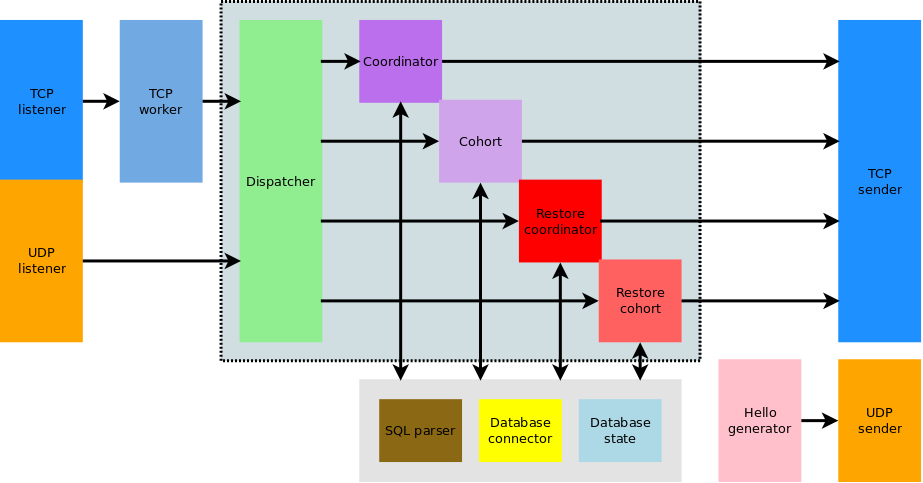
\includegraphics[width=22cm,angle=90]{architektura.png}
\caption{Architektura rozwiązania}
\end{figure}
\pagebreak

\chapter{Trójfazowe zatwierdzanie transakcji}
Główną częścią logiki systemu będzie trójfazowe zatwierdzanie transakcji, które umożliwi wykonanie pojedynczej transakcji na wszystkich lub na żadnym węźle. Poniżej opis protokołu.
\section{Model automatowy}
\subsubsection{Serwer (Coordinator)}
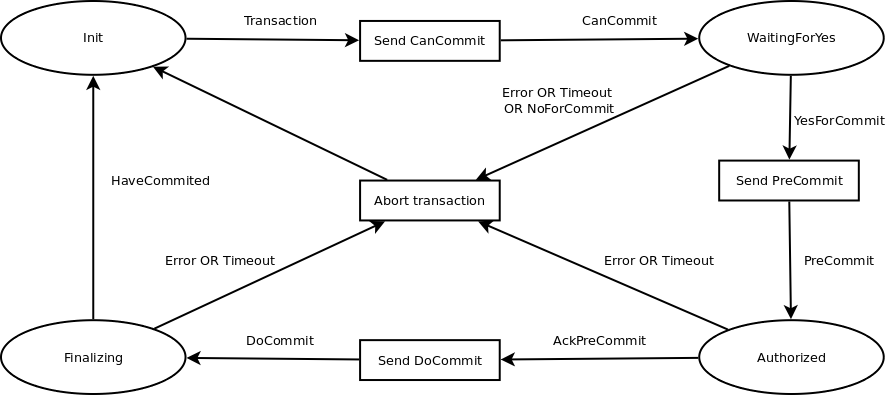
\includegraphics[width=15cm]{3PC-serwer.png}
\subsubsection{Klient (Cohort)}
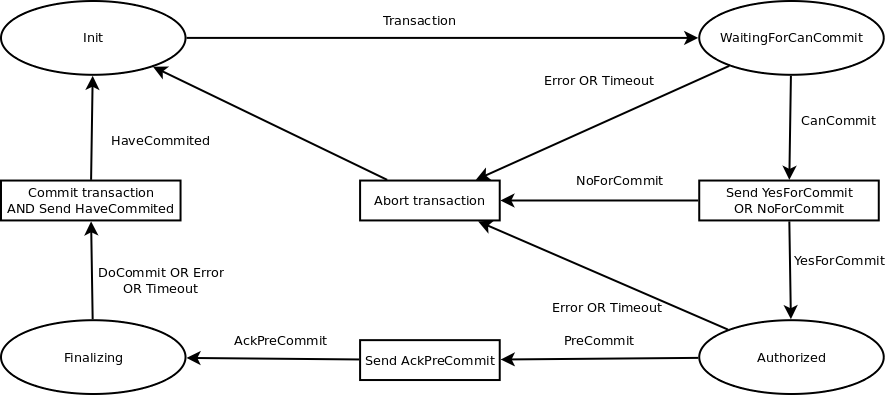
\includegraphics[width=15cm]{3PC-klient.png}
\section{Opis słowny}
Zatwierdzanie trójfazowe jest rozproszonym algorytmem, który nakazuje węzłą w rozproszonym systemie uzgodnić fakt zatwierdzania transakcji. W przeciwieństwie do swojego dwufazowego poprzednika, wersja trójfazowa jest nieblokująca. 

\subsubsection{Serwer (Coordinator)}
\begin{enumerate}
	\item Pewien klient inicjuje sekwencję trójfazowego zatwierdzenia za pomocą pakietu \verb+Transaction+. W razie problemu transakcja jest anulowana. Koordynator wysyła zapytanie do klientów, czy chcą zatwierdzić (\verb+CanCommit+) i przechodzi do stanu oczekiwania. 
	\item W przypadku odpowiedzi pozytywnej wysyła do wszystkich wiadomość \verb+PreCommit+, który nakazuje stacjom klienckim przygotować się do zatwierdzenia. W razie błędu, upłynięcia limitu czasu dla którejś ze stacji lub odebrania od dowolnego klienta \verb+NoForCommit+ - transakacja jest anulowana. W przeciwnym wypadku następuje trzecia faza
	\item W~trzeciej fazie kordynator wysyła \verb+DoCommit+, który ostatecznie nakazuje klientom zatwierdzić lub odrzucić daną transakcję. Gdyby w którejś fazie nie dotarł pakiet - klient lub serwer odczekują określony czas i ewentualnie anulują transakcję.
\end{enumerate}
\subsubsection{Klient (Cohort)}
\begin{enumerate}
	\item Klient dostaje zapytanie, czy chce zatwierdzić transakcję i odpowiada twierdząco (komunikat \verb+YesForCommit+) i przechodzi do stanu przygotowania, ewentualnie odpowiada, że chce transakcję odrzucić (komunikat \verb+NoForCommit+).
	\item W stanie przygotowania, jeśli dostanie komunikat o anulowaniu lub minie timeout, transakcja jest anulowana. Jeśli otrzyma komunikat \verb+PreCommit+ potwierdza go komunikatem \verb+AckPreCommit+.
	\item Po odebraniu komunikatu \verb+DoCommit+ transakcja jest zatwierdzana (i wysyłany jest komunikat \verb+HaveCommitted+), w przeciwnym wypadku (błąd lub upłynięcie timeoutu transakcja jest anulowana).
\end{enumerate}

\chapter{Dynamiczne dodawanie nowych węzłów}
\begin{figure}[h]
\centering
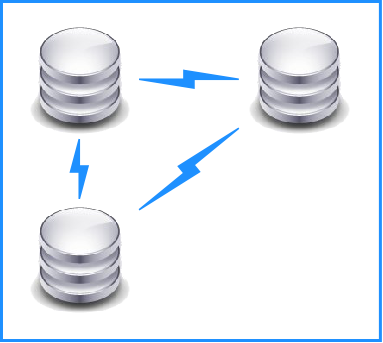
\includegraphics[height=8cm]{restore_init.png}
\caption{Początkowa faza - 3 węzły działające}
\end{figure}

\begin{figure}[h]
\centering
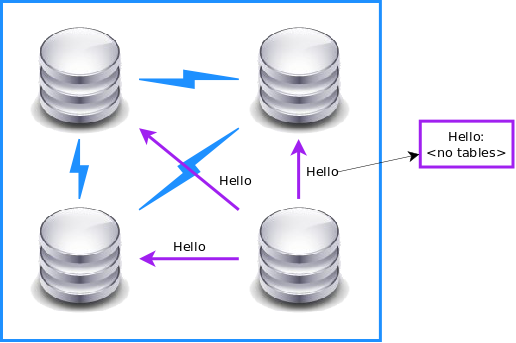
\includegraphics[height=8cm]{restore_first_hello.png}
\caption{Nowo dodany węzeł zaczyna rozgłaszać swoje Hello}
\end{figure}

\begin{figure}[h]
\centering
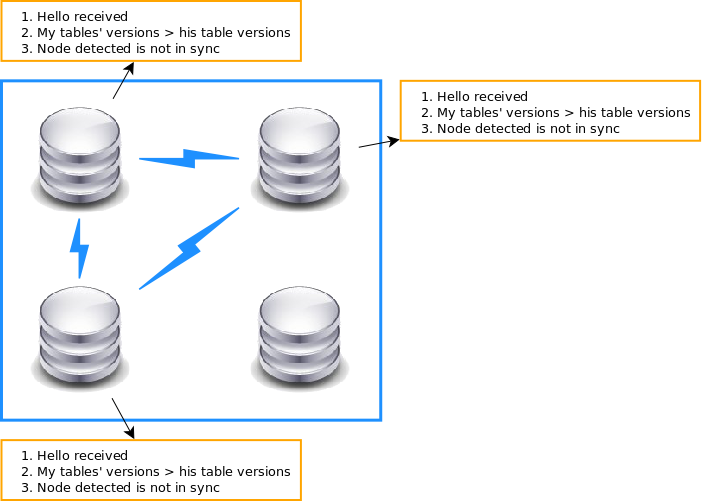
\includegraphics[height=12cm]{restore_node_not_in_sync.png}
\caption{Obecne węzły porównują tabele w pakiecie Hello z własnymi wersjami i stwierdzają, że konieczna jest synchronizacja}
\end{figure}

\begin{figure}[h]
\centering
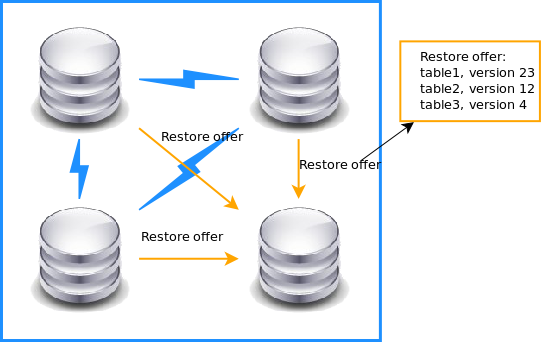
\includegraphics[height=8cm]{restore_restore_offer.png}
\caption{Węzły blokują odpowiednie obszary danych, a gdy ich listy prowadzonych sesji będą puste, wysyłana jest oferta synchronizacji}
\end{figure}

\begin{figure}[h]
\centering
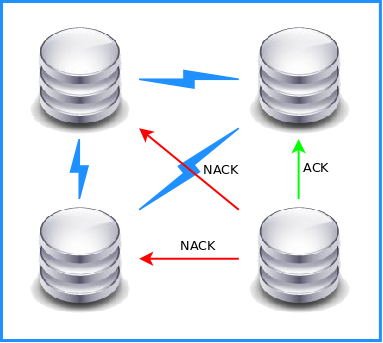
\includegraphics[height=8cm]{restore_restore_ack.png}
\caption{Nowy węzeł wybiera jeden z węzłów do synchronizacji, pozostałe odrzuca}
\end{figure}

\begin{figure}[h]
\centering
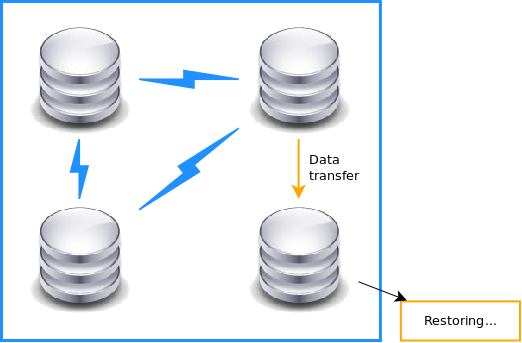
\includegraphics[height=8cm]{restore_restore_data_transfer.png}
\caption{Następuje transfer tabel i synchronizacja danych}
\end{figure}

\begin{figure}[h]
\centering
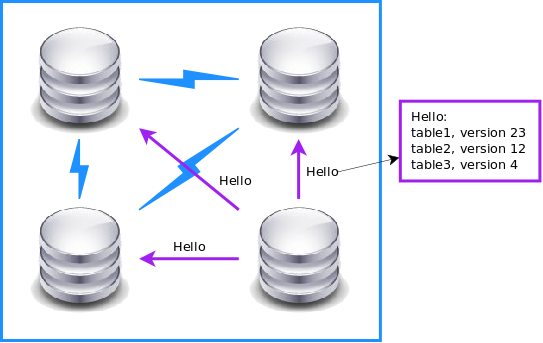
\includegraphics[height=8cm]{restore_after_sync_hello.png}
\caption{Po synchronizacji węzeł będzie wysyłał już hello z poprawnymi wersjami tabel}
\end{figure}

\begin{figure}[h]
\centering
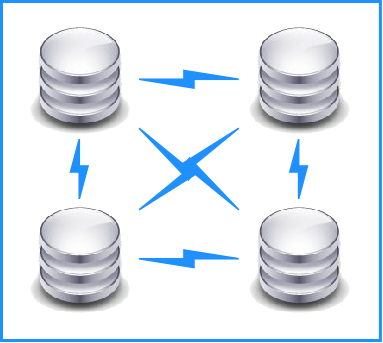
\includegraphics[height=8cm]{restore_connected.png}
\caption{Ostatecznie zostanie uznany za zsynchronizowany i włączony do struktury}
\end{figure}

\chapter{Diagramy sekwencji}
\section{Wiadomości}
Poniżej zaprezentowane zostały diagramy sekwencji wywołań metod w klasach używanych do trójfazowego zatwierdzania transakcji. Aby wszystkie diagramy były zrozumiane na początku zaprezentowano hierarchię klas dla TPC oraz przedstawiające hierarchie klas stanów Coordinatora i Cohort'a.
\begin{figure}[h]
\centering
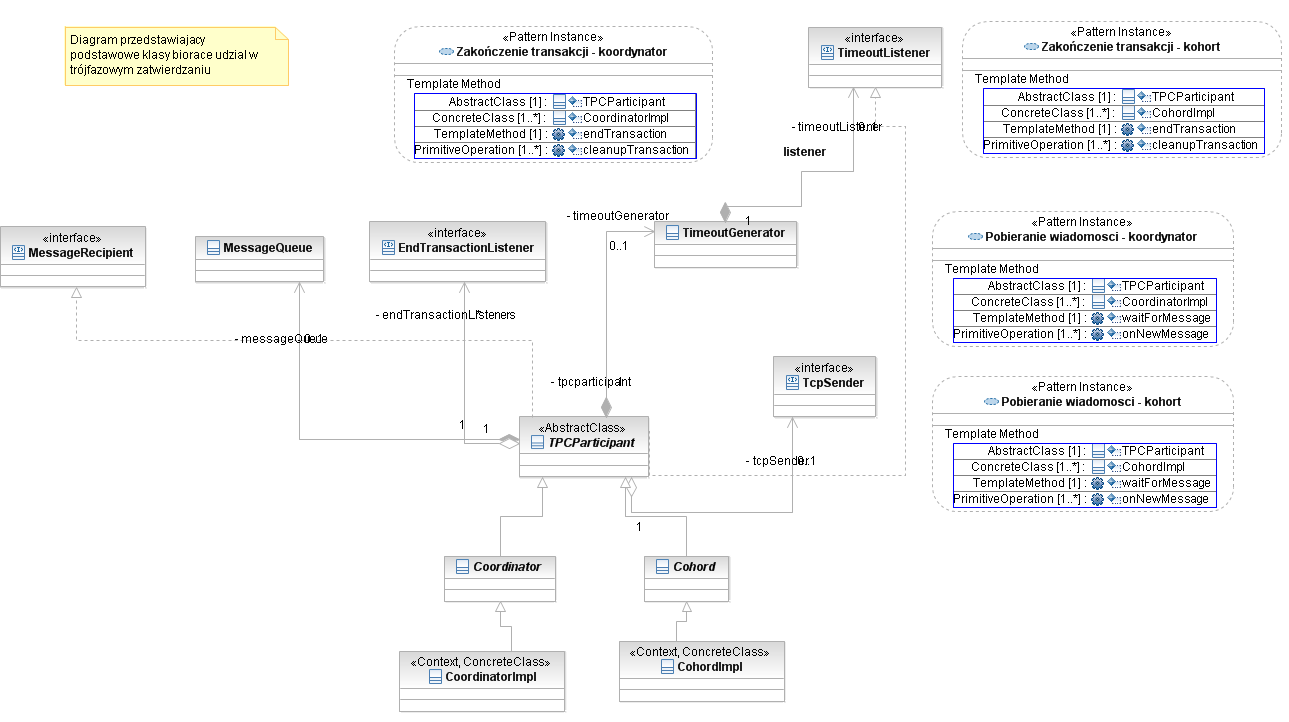
\includegraphics[width=22cm,angle=90]{sekwencje/TPC.png}
\caption{Ogólna hierarchia klas dla TPC}
\end{figure}

\begin{figure}[h]
\centering
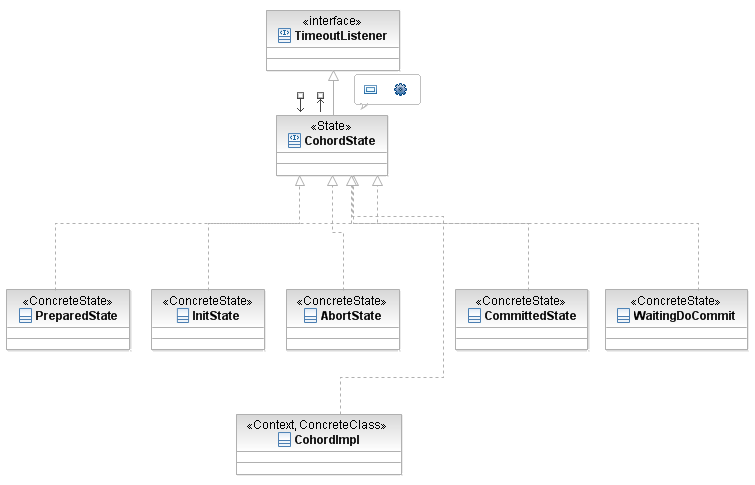
\includegraphics[width=15cm]{sekwencje/CohCohordStates.png}
\caption{Hierarchia klas dla Cohort}
\end{figure}


\begin{figure}[h]
\centering
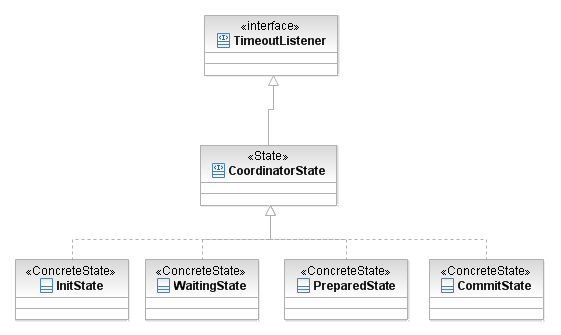
\includegraphics[width=15cm]{sekwencje/CorCoordinatorStates.png}
\caption{Hierarchia klas dla Coordinator}
\end{figure}


\begin{figure}[h]
\centering
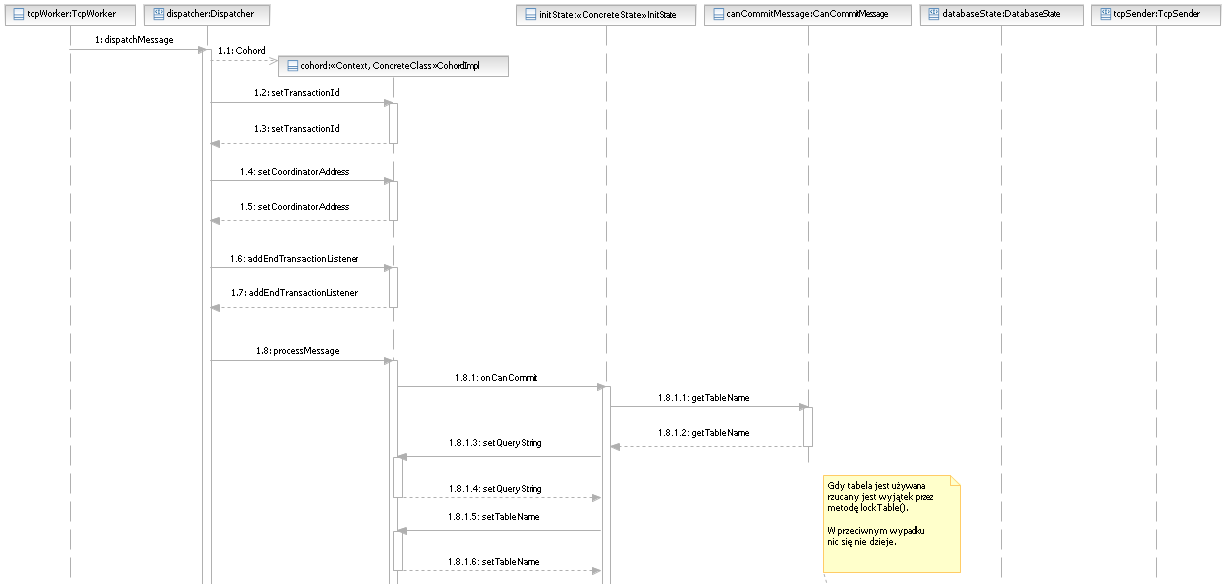
\includegraphics[width=22cm,angle=90]{sekwencje/CanCommitMessage1.png}
\caption{Obsługa wiadomości CanCommit - cz. 1}
\end{figure}


\begin{figure}[h]
\centering
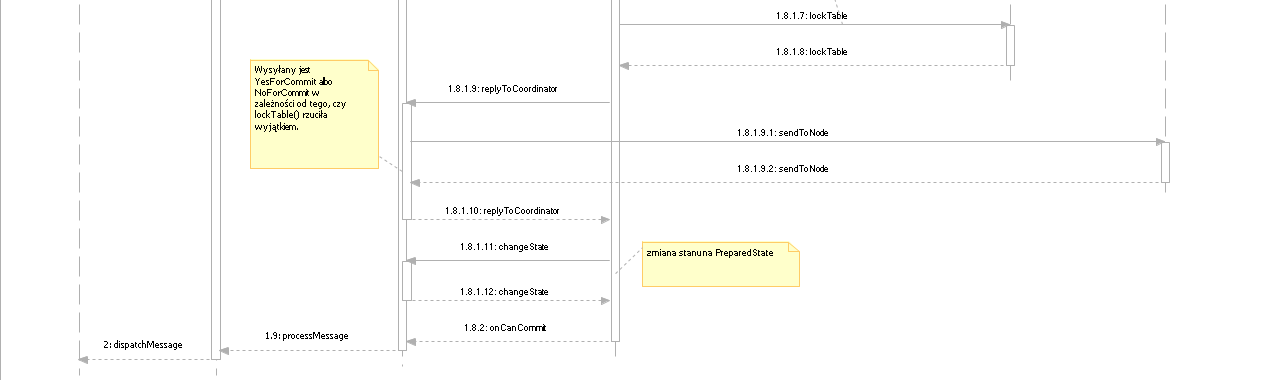
\includegraphics[width=22cm,angle=90]{sekwencje/CanCommitMessage2.png}
\caption{Obsługa wiadomości CanCommit - cz. 1}
\end{figure}

\begin{figure}[h]
\centering
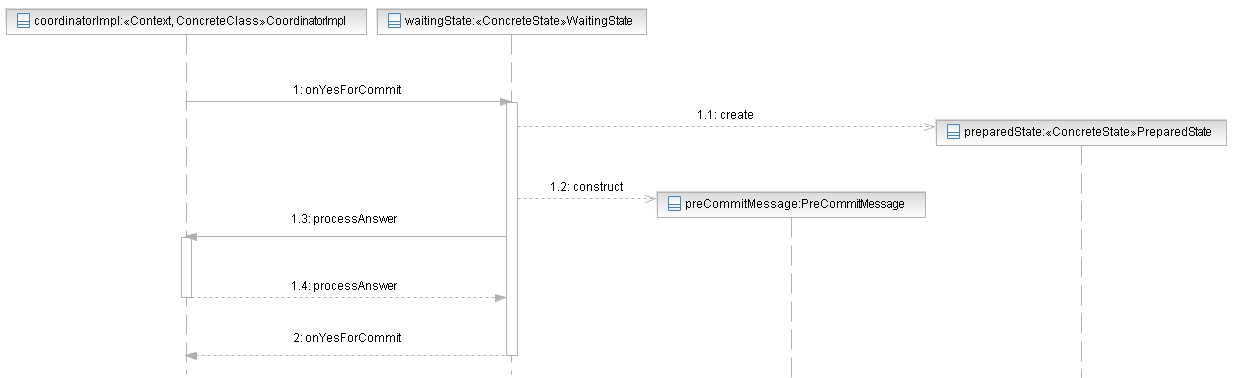
\includegraphics[width=22cm,angle=90]{sekwencje/YesForCommit.png}
\caption{Obsługa wiadomości YesForCommit}
\end{figure}

\begin{figure}[h]
\centering
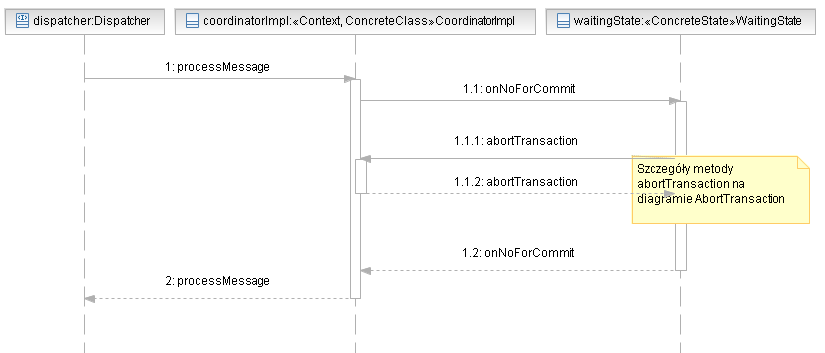
\includegraphics[width=22cm,angle=90]{sekwencje/NoForCommit.png}
\caption{Obsługa wiadomości NoForCommit}
\end{figure}

\begin{figure}[h]
\centering
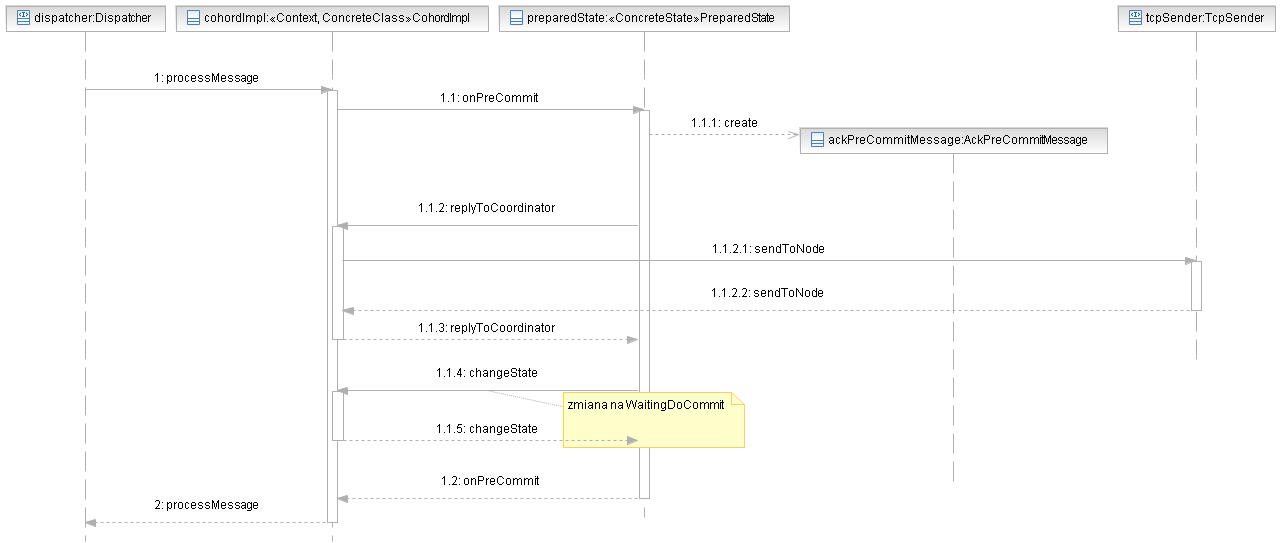
\includegraphics[width=22cm,angle=90]{sekwencje/PreCommitMessage.png}
\caption{Obsługa wiadomości PreCommit}
\end{figure}

\begin{figure}[h]
\centering
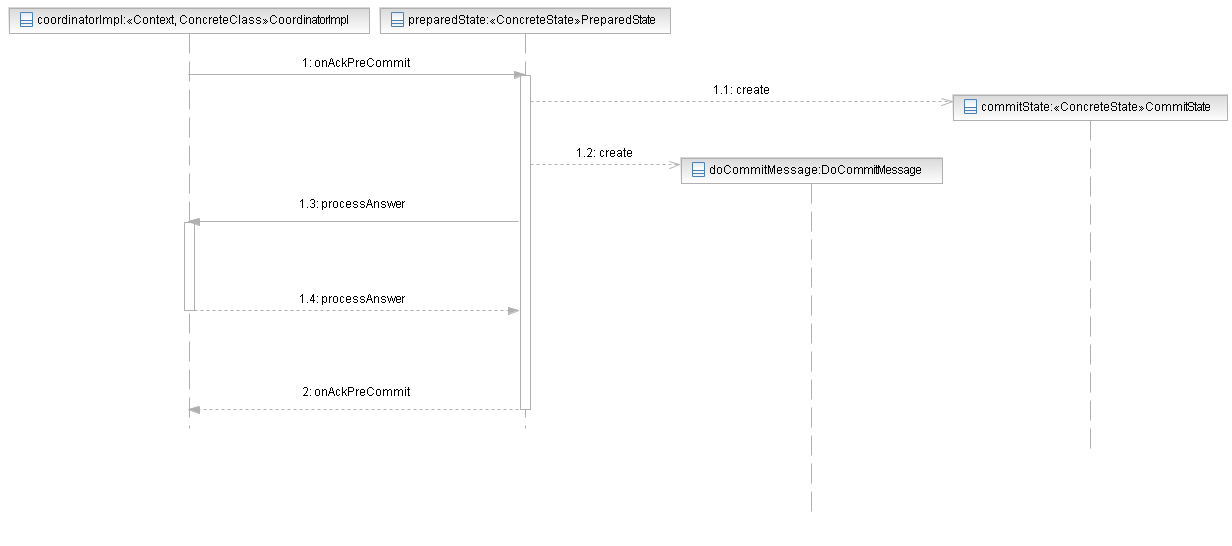
\includegraphics[width=22cm,angle=90]{sekwencje/AckDoCommitMessage.png}
\caption{Obsługa wiadomości AckPreCommit}
\end{figure}

\begin{figure}[h]
\centering
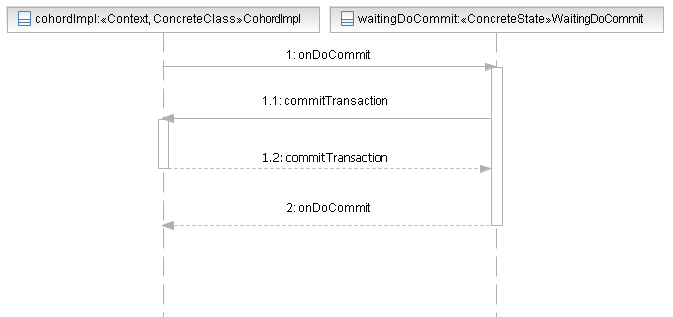
\includegraphics[width=22cm,angle=90]{sekwencje/DoCommitMessage.png}
\caption{Obsługa wiadomości DoCommit}
\end{figure}

\begin{figure}[h]
\centering
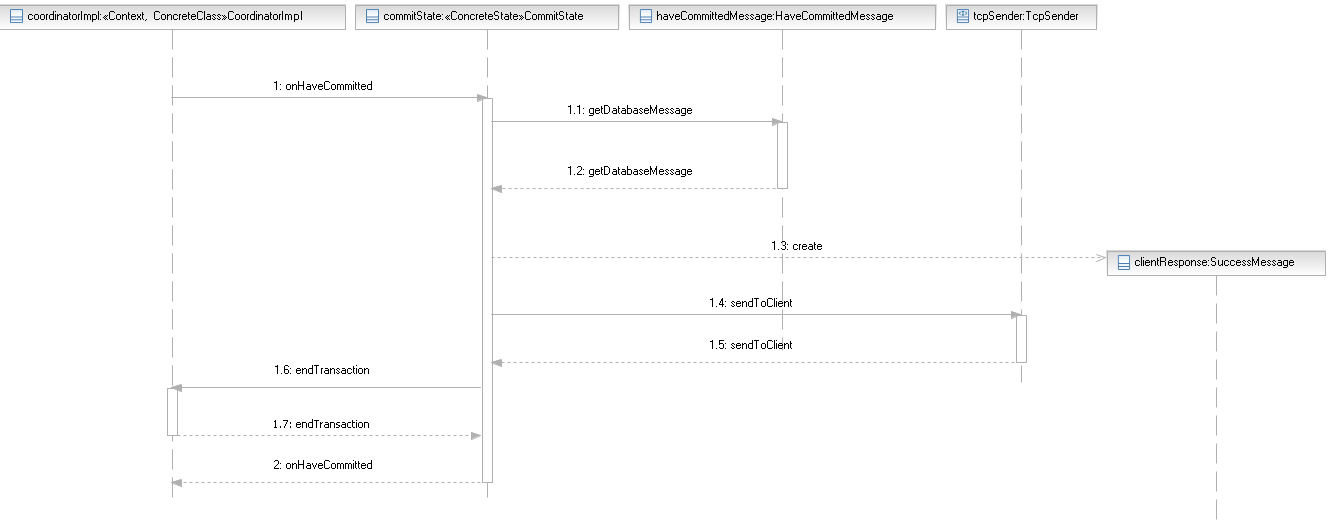
\includegraphics[width=22cm,angle=90]{sekwencje/HaveCommittedMessage.png}
\caption{Obsługa wiadomości HaveCommitted}
\end{figure}
\end{document}
